\chapter{Reactive programming}\label{reactive-programming}

When using the imperative programming paradigm, the act of capturing
dynamic values is done only indirectly, through \textbf{state and
mutations}. In this context, the idea of \emph{dynamic/evolving} values
is not a first class value in the paradigm. Moreover, the paradigm can
only capture discrete evolving values, since the paradigm itself is
\emph{temporally discrete}.

Reactive programming is a programming paradigm that aims to provide a
more declarative way to abstract computations and mutations.

Wikipedia defines reactive programming as: 
\begin{quote} 
a programming paradigm oriented around data flows and the propagation of change. This
means that it should be possible to express static or dynamic data flows
with ease in the programming languages used, and that the underlying
execution model will automatically propagate changes through the data
flow.
\end{quote}

In this definition emerges some key concepts: 

\begin{itemize}
\itemsep1pt\parskip0pt\parsep0pt
\item
  expressing computations in terms of \textbf{data flows} 
\item
  \textbf{change is propagated} in a composable way 
\item
  the language or framework has to support \textbf{declarativeness} 
\item
  all the ``plumbing work'' is done by the execution model, ensuring that the actual 
  computation respects the semantics

\end{itemize}

One of the best examples to describe reactive programming is to think of
a spreadsheet, in which there're three cells, A, B and C and A is
defined as the sum of B and C. Whenever B or C changes, A updates
itself. The example is really simple and it's also something that we're
used to know. Reactive programming is all about propagating changes
throughout a system, automatically.

This chapter will focus on \textbf{Functional Reactive Programming} and
\textbf{Reactive Programming}, in an attempt to provide formal
definitions.

\section{Functional Reactive
Programming}\label{functional-reactive-programming}

Functional reactive programming has its origin with \emph{Fran}
(Functional reactive animation), a Haskell library for interactive
animations by Conal Elliott. Elliott found it difficult to express the
\emph{what} of an interactive animation abstracting from the \emph{how},
and built a set of expressive and recursive data types, combined with a
declarative programming language.

Informally, \textbf{functional reactive programming} is a programming
paradigm which brings a notion of \textbf{time} in the functional
programming paradigm, providing a conceptual framework for implementing
reactive systems. Infact, FRP let the application achieve reactivity by
providing constructs for specifying \emph{how behaviors change in
response to events}.

Elliott says that FRP is all about two main things: \emph{denotative}
and \emph{temporally continuos}. Infact, he also likes the term
``\emph{denotative, continuos-time programming}'' to replace functional
reactive programming, since it reduces the confusion.

Always about the \textbf{denotative} part, he means that the paradigm
should be founded on a precise, simple, implementation-independent,
compositional semantics that exactly specifies the meaning of each type
and building block. The compositional nature of the semantics then
determines the meaning of all type-correct combinations of the building
blocks.

From an Elliott's quote: 

\begin{quote}
Denotative is the heart and
essence of functional programming, and is what enables precise and
tractable reasoning and thus a foundation for correctness, derivation,
and optimization.
\end{quote}

About the \textbf{continuous time} part, there's some confusion. Some
claim that it's an idea somehow unnatural or impossible to implement
considering the discrete nature of computers. To this issues, Elliott
answers in the following way:

\begin{quote}
This line of thinking strikes me as bizarre, especially when coming from
Haskellers, for a few reasons: Using lazy functional languages, we
casually program with infinite data on finite machines. We get lovely
modularity as a result {[}\ldots{}{]}. There are many examples of
programming in continuous space, for instance, vector graphics,
{[}\ldots{}{]} I like my programs to reflect how I think about the
problem space rather than the machine that executes the programs, and I
tend to expect other high-level language programmers to share that
preference.
\end{quote}

Another name that Elliott suggests for continuous is
\emph{resolution-independent}, and thus able to be transformed in time
and space with ease and without propagating and amplifying sampling
artifacts. As an example, he propose the ``finite vs infinite'' data
structure issue:

\begin{quote}
We only access a finite amount of data \emph{in the end}. However,
allowing infinite data structures \emph{in the middle} makes for a much
more composable programming style. Each event has a stream (finite or
infinite) of occurrences. Each occurrence has an associated time and
value.
\end{quote}

Fran integrates general ideas from synchronous data-flow languages into
the non-strict, pure functional language Haskell. It takes a monadic
approach and encapsulates operations over time-varying values and
discrete events into data structures that are evaluated by an
interpreter loop. The main idea of FRP is to model user inputs as
functions that changes over time.


\subsection{Behaviors and Event Streams}\label{behaviors-and-event-streams}

FRP introduces two special abstractions:

\begin{itemize}
\itemsep1pt\parskip0pt\parsep0pt
\item
  \textbf{behaviors or signals}, values that are continuos functions of
  time.
\item
  \textbf{event streams}, values which are discrete functions of time.
\end{itemize}

\textbf{Behaviors} are dynamic/evolving values, and are first class
values in themselves. Behaviors can be defined and \emph{combined}, and
\emph{passed} into and out of functions.

Behaviors are built up out of a few primitives, like constant (static)
behaviors and time (like a clock), and then with sequential and parallel
combination. n-behaviors are combined by applying an n-ary function (on
static values), ``point-wise'', i.e., continuously over time.

In other terms, a Behavior simply \textbf{sends values over time} until
it either \textbf{completes}, or \textbf{errors out}, at which point it
stops sending values forever.

Examples of behaviours are the following:

\begin{itemize}
\itemsep1pt\parskip0pt\parsep0pt
\item
  time
\item
  a browser window frame
\item
  the cursor position
\item
  the position of a image during an animation
\item
  audio data
\item
  \ldots{}
\end{itemize}

\textbf{Events} enable to account for discrete phenomena, and each of it
has a stream (finite or infinite) of occurrences. Each occurrence is a
value paired with a time. Events are considered \emph{to be improving
list of occurences}.

Formally, the points at which an event stream is defined are termed
\emph{events} and events are said to \emph{occur} on an \emph{event
stream}.

Example of event streams are the following:

\begin{itemize}
\itemsep1pt\parskip0pt\parsep0pt
\item
  timer events
\item
  key presses
\item
  mouse clicks
\item
  MIDI data
\item
  network packets
\item
  \ldots{}
\end{itemize}

Every instance of FRP conceptually includes both behaviors and events.
The classic instance of FRP takes behaviors and events as first-class
values.

\section{Evaluation model}\label{evaluation-model}

The core of languages that support Reactive Programming is about
\textbf{how changes are propagated}. From the programmer's point of view
this should be as much transparent as possible. In other words, a change
of a value is automatically propagated to all dependent computations
without the user has to manually propagate the changes by himself.

At the language level this means that there should be a mechanism that
is triggered when there's an event occurence at an event source. This
mechanism will fire a notification about the changes to dependent
computations, that will possibly trigger a recomputation, and so on.

The issue of \emph{who initiates the propagation of changes} is a really
important decision in designing a language or a framework that supports
RP.

In simple terms the question is whether the source should \emph{push}
new data to its dependents (consumers) or the dependents should
\emph{pull} data from the event source (producer).

\begin{figure}[htbp]
\centering
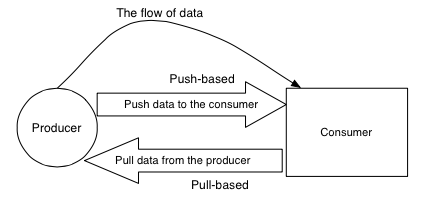
\includegraphics[scale=0.75]{imgs/eval.png}
\caption{Push- Versus Pull-based evaluation model, from the paper ``A
survey on Reactive Programming''}
\end{figure}

In the literature there are two main evaluation models:

\begin{itemize}
\itemsep1pt\parskip0pt\parsep0pt
\item
  \textbf{Pull-Based}, in which the computation that requires a value
  has to pull it from the source. The propagation is said to be
  \emph{demand-driven}. The pull model has been implemented in Fran,
  also thanks to the lazy evaluation of Haskell. A main trait of this
  approach is that the computation requiring the value has the liberty
  to only pull the new values when if actually needs it. From another
  point of view, this trait can lead to a significant latency between an
  occurence of an event and when its reactions are triggered.
\item
  \textbf{Push-Based}, in which when the event source has new data it
  pushes the data to its dependent computations. The propagation is said
  to be \emph{data-driven}. An example of a recent implementation that
  use this model is Scala.React, that will be introduced later in this
  thesis. This approach also brings the issue of wasteful recomputation,
  since every new data that is pushed to the consumer triggers a
  recomputation.
\end{itemize}

Tipically, reactive programming languages use \textbf{either a
pull-based or push-based model}, but there are also languages that
employ \textbf{both} approaches. In latter case there've both the
benefits of the push-based model (efficiency and low latency) and those
of the pull-based model (flexibility of pulling values based on demand).

\section{Glitches}\label{glitches}

A \textbf{glitch} is a \textbf{temporary inconsistency} in the
observable state. Due to the fact that updates do not happen
instantaneously, but instead take time to compute, the values within a
system may be \textbf{transiently out of sync} during the update
process. This may be a problem, depending on how tolerant the
application is of occasional stale inconsistent data. For example,
consider a computation that is run before all its dependent expressions
are evaluated and that can result in fresh values being combined with
stale values.

The paper ``A Survey on Reactive Programming'' by Bainomugisha et al.
depict the problem with the following program:

\begin{verbatim}
var1 = 1
var2 = var1 * 1
var3 = var1 + var2
\end{verbatim}

\begin{figure}[htbp]
\centering
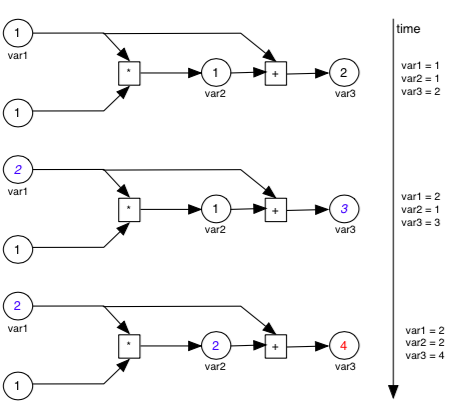
\includegraphics[scale=0.75]{imgs/glitches.png}
\caption{Momentary view of inconsistent program state and
recomputation.}
\end{figure}

The image related to the program above shows how the state of the
program results incorrect (\texttt{var3} is evaluated as 3 instead of 4)
and that this also leads to a wasteful recomputation (since
\texttt{var3} is computed one time more than the necessary).

Glitches only happens when using a \emph{push-based} evaluation model
and can be avoided by arranging expressions in a topologically sorted
graph. This implementation detail ensures that an expression is always
evaluated after all its dependants have been evaluated.

\section{Lifting}\label{lifting}

The term \emph{lifting} is used to depict the process of
\textbf{converting} an ordinary operator to a variant that can operate
on behaviors. This process is essential for the end user of the
language/framework, since it ensures conciseness and composability. In
other words, lifting is used to move from the non-reactive world to
reactive behaviors.

Lifting a \textbf{value} creates a \textbf{constant behavior} while
lifting a \textbf{function} \textbf{applies the function continuously}
to the argument behaviors. There is no similar lifting operation for
events, since an event would need an occurrence time as well as a value.

Lifting an operation can be formalized by the following definition,
assuming functions that only take one parameter (generalising to
functions that take multiple arguments is trivial):

\[
lift: f(T)  \rightarrow f_{lifted} (Behavior < T >).
\]

The \(f_{lifted}\) function can now be applied to behaviors that holds
values of type \(T\). Lifting enables the language or framework to
register a dependency graph in the application's dataflow graph.

Starting from the previous definition, the evaluation of a lifted
function called with a behavior at the time step \(i\) can be formalized
as follows:

\[
f_{lifted}(Behavior < T >)  \rightarrow f(T_i) .
\]

where \(T_i\) is the value of the behavior at the time step \(i\).


In the literature there are at least three main lifting strategies:

\begin{enumerate}
\def\labelenumi{\arabic{enumi}.}
\item
  \textbf{Implicit lifting}, that happens when an ordinary language
  operator is applied on a behaviour and it is automatically lifted.
  Implicit lifting is often used by dynamically typed languages.
  Formally: \[
  f(b1)  \rightarrow f_{lifted}(b1) .
  \]
\item
  \textbf{Explicit lifting}, usually used by statically typed languages.
  In this case the language provides a set of combinators to lift
  ordinary operators to operate on behaviors. Formally: \[
  lift(f)(b1)  \rightarrow f_{lifted}(b1) .
  \]
\item
  \textbf{Manual lifting}, when the language does not provide lifting
  operators. Formally: \[
  f(b1)  \rightarrow f(currentValue(b1)) .
  \]
\end{enumerate}


\section{Reactive confusion}\label{reactive-confusion}

In these days \textbf{reactive programming} and \textbf{functional
reactive programming} are two terms that create a lot of
\textbf{confusion}, and maybe are also over-hyped.

The definitions that come from Wikipedia are still pretty vague and only
Functional reactive programming introduced by Connal Elliott has a clear
and simple denotative semantics. In advance to this, Elliott himself
doesn't like the name he gave to the paradigm.

The concepts behind these newly introduced paradigms are prerry similar.
Reactive programming is a paradigms that facilitates the development of
applications by providing \textbf{abstractions} to express
\emph{time-varying values} and automatically propagating the
\emph{changes}: behaviors and events. Functional reactive programming
can be considered a ``sibiling'' of reactive programming, providing
composable abstractions. Elliot identifies the key advantages of the
functional reactive programming paradigm as: \emph{clarity, ease of
construction, composability, and clean semantics}.

In 2013 Typesafe launched http://www.reactivemanifesto.org, which tried
to define what reactive applications are. The reactive manifesto didn't
introduce a new programming paradigm nor depicted RP as we intended RP
in this thesis. What the reactive manifesto did instead was to depict
some really relevant computer science principles about scalability,
resilience and event-driven architectures, and RP is one of the tools of
the trade.

Erik Meijer, in his talk ``Duality and the End of Reactive'', concluded
that all the hype and the buzzwords around the ``reactive world'' has no
sense, and that the core of the paradigm is \textbf{all about composing
side effects}. In his talk and related papers, he depicted the
\textbf{duality} that links enumerables and observables.

\begin{table}[]
\centering
\caption{The essential effects in programming}
\label{my-label}
\begin{tabular}{|l|l|l|}
\hline
             & {\bf One}     & {\bf Many}        \\ \hline
Synchronous  & T/Try{[}T{]}  & Iterable{[}T{]}   \\ \hline
Asynchronous & Future{[}T{]} & Observable{[}T{]} \\ \hline
\end{tabular}
\end{table}

In short, an enumerator is basically a getter with the ability to fail
and/or terminate. It might also return a future rather than a value. An
\textbf{iterable} is a getter that returns an \textbf{iterator}. If we
take the category-theoretic dual of these types we get the
\textbf{observer} and \textbf{observable} types. And this conclusion is
what let us to relate all the principal effects in programming, where in
one axis there's is the nature of the computation (sync or async) and in
the other one there's the cardinality of the result (one or many).
